\documentclass[aspectratio=159]{beamer}

\usepackage{bm}
\usetheme{metropolis}           % Use metropolis theme
\title{An Introduction to PAC-Bayes Bounds}
\date{\today}
\author{Luis A. Ortega}
\institute{Universidad Autónoma de Madrid}
\usepackage[most]{tcolorbox}

\NeedsTeXFormat{LaTeX2e}
\usepackage{amsfonts}       % blackboard math symbols
\usepackage{amssymb,amsmath,amsthm}
\usepackage{braket}
\usepackage{booktabs} % for professional tables
\usepackage{tabularx}
\usepackage{multirow}
\usepackage{centernot}

\usefonttheme{professionalfonts} % required for mathspec
\usepackage{mathspec}

\usepackage[sfdefault,light,lining]{FiraSans} 
\usepackage[natbib=true, backend=biber, style=authoryear-icomp, useprefix=true]{biblatex}
\addbibresource{refs.bib}

\newcommand{\h}[1]{\color{orange}\textbf{#1}}

\DeclareMathOperator*{\argmax}{arg\,max}
\DeclareMathOperator*{\argmin}{arg\,min}

\colorlet{shadecolor}{gray!40}
\begin{document}
    \maketitle


    \begin{frame}{}
        In a \textbf{supervised learning} problem, we are given a data set, and 
        \begin{enumerate}
            \item Fix a family of predictors.
            \item Find a good predictor in this set.
        \end{enumerate}
        \pause
        For example, for \textbf{linear regression}, you 1) choose to consider only \textbf{linear predictors} and 2) use the \textbf{least-square method} to choose your linear predictor.
    \end{frame}

    \begin{frame}{Notation I}
        The objective is to \textit{\textbf{learn from examples to assign labels to objects}}. \pause
        \begin{itemize}[<+->]
            \item The set of all possible objects will be denoted by \(\mathcal{X} \subset \mathbb{R}^d\) . 
            \item The set of labels will be denoted by \(\mathcal{Y}\).
            \item A predictor is a function \(f : \mathcal{X} \to \mathcal{Y}\). We are usually interested in parametric sets of predictors. That is, we consider \(\{f_{\theta}, \theta \in \Theta\}\).
            \item A loss function \(\ell : \mathcal{Y}^2 \to [0, + \infty)\); where \(\ell(y, y) = 0 \).
            The \(0-1\) loss for classification:
            \[
                \ell(y, y') = \begin{cases}
                    0 & \text{ if } \quad y = y'\,,\\
                    1 & \text{ if } \quad y \neq y'\,.
                \end{cases}
            \]
        \end{itemize}
    \end{frame}

    \begin{frame}{Notation II}
        We want to \textbf{predict the label of objects} in the future.\pause
        \begin{itemize}[<+->]
            \item Let \(P\) denote the probability distribution over \(\mathcal{X} \times \mathcal{Y}\). 
            \item The \textbf{expected error} (generalization risk) is 
            \[
                R(f) := \mathbb{E}_{(X, Y) \sim P}[\ell(f(X), Y)]\,, \quad R(\theta) := R(f_\theta)\,.
            \]
            \item Observations, \(S := [(X_1, Y_1),\dots , (X_n, Y_n)] \) are i.i.d from \(P\).
            \item The \textbf{empirical risk}:
            \[r(\theta) = \tfrac{1}{n}\sum_{i=1}^n \ell(f_\theta(X_i), Y_i), \quad \mathbb{E}_{S}[r(\theta)] = R(\theta)\,.\]
        \end{itemize}
    \end{frame}
    \begin{frame}{Notation III}
            An \textbf{estimator} takes observations and returns a predictor:
            \[
                \hat{\theta}: \bigcup_{n=1}^{\infty}(\mathcal{X} \times \mathcal{Y})^n \to \Theta\,.
            \]\pause
            For example, the \textbf{empirical risk minimizer (ERM)}:
            \[
                \hat{\theta}_{ERM} = \argmin_{\theta \, \in \, \Theta} r(\theta) = \argmin_{\theta \, \in\,  \Theta} \tfrac{1}{n}\sum_{i=1}^n \ell(f_\theta(X_i), Y_i)\,.
            \]
    \end{frame}

    \begin{frame}{PAC Bounds}
        \[
        \hat{\theta}_{ERM} = \argmin_{\theta \, \in \, \Theta} r(\theta) \centernot \implies \hat{\theta}_{ERM} = \argmin_{\theta \, \in \, \Theta} R(\theta)\,.
        \]

        ERM relies on the \textit{hope} that ``\textit{these two functions are not so different}''. \pause

        \textbf{Proposition 1.} If \(\ell(\cdot, \cdot)\) is \textbf{bounded} in [0, C]; for any \(\theta \in \Theta\) and \(\delta \in (0,1)\), 
        \[
        \mathbb{P}_{S}\left[ R(\theta) > r(\theta) + C\sqrt{\frac{\log \frac{1}{\delta}}{2n}} \right] \leq \delta \pause \iff \mathbb{P}_{S}\left[ R(\theta) \leq r(\theta) + C\sqrt{\frac{\log \frac{1}{\delta}}{2n}} \right] \geq 1- \delta\,.
        \]  
        \textit{Proof. } Hoeffding’s inequality to \(U_i = \mathbb{E}[\ell_i(\theta)] - \ell_i(\theta)\).
    \end{frame}

    \begin{frame}
        \textbf{Proposition 1.} If \(\ell(\cdot, \cdot)\) is \textbf{bounded} in [0, C]; for any \(\theta \in \Theta\) and \(\delta \in (0,1)\), 
        \[
            \mathbb{P}_{S}\left[ R(\theta) > r(\theta) + C\sqrt{\frac{\log \frac{1}{\delta}}{2n}} \right] \leq \delta  \pause \iff \mathbb{P}_{S}\left[ R(\theta) \leq r(\theta) + C\sqrt{\frac{\log \frac{1}{\delta}}{2n}} \right] \geq 1- \delta\,. 
        \]
        \pause
        \begin{enumerate}[<+->]
            \item Proposition 1 states that \(R(\theta)\) will ``usually'' not exceed \(r(\theta)\) by more than a term in \(1/\sqrt{n}\). 
            \item This is \textbf{not enough}, to justify the use of the ERM. 
            \item The result is only true for a \textbf{fixed} \(\theta\), and we cannot apply it to \(\hat{\theta}_{ERM}\) that is a function of the data.
        \end{enumerate}
    \end{frame}

    \begin{frame}{PAC Bound on ERM}
        The usual approach to control \(R(\hat{\theta}_{ERM})\) is to use:
        \[
        R(\hat{\theta}_{ERM}) - r(\hat{\theta}_{ERM}) \leq \sup_{\theta \in \Theta} R(\theta) - r(\theta)\,.
        \]

        \textbf{Theorem 2. }Assume that \(\Theta = \{\theta_1, \dots, \theta_M\}\). Then, for any \(\delta \in (0,1)\),
        \[
            \mathbb{P}_{S}\left[ R(\hat{\theta}_{ERM}) \leq \inf_{\theta \in \Theta} r(\theta) + C \sqrt{\frac{\log \tfrac{M}{\delta}}{2n}} \right] \geq 1- \delta\,.
        \]
        \pause
        \begin{center}
        These are called \textbf{Probably Approximately Correct (PAC) Bounds}.
        \end{center}
        \[
        r(\hat{\theta}_{ERM}) = \inf_{\theta \in \Theta} r(\theta) \text{ approximates } R(\hat{\theta}_{ERM}) \text{ within }C\sqrt{\frac{\log\tfrac{M}{\delta}}{2n}} \text{ with prob. } 1 - \delta\,.
        \]
    \end{frame}

    {\setbeamercolor{background canvas}{bg=white}
    \begin{frame}{PAC Bound Example}
    \begin{center}
        \[
            \mathbb{P}_{S}\left[ R(\hat{\theta}_{ERM}) \leq \inf_{\theta \in \Theta} r(\theta) + C \sqrt{\tfrac{\log \tfrac{M}{\delta}}{2n}} \right] \geq 1- \delta\,.
        \]
    \end{center}
    \begin{minipage}{0.5\textwidth}
        Let \(\min_{\theta \in \Theta} r(\theta) = 0.26\), \(C = 1\), \(M = 100\), \(n = 1000\) and  \(\delta = 0.05\)
        \[
            \mathbb{P}_S\left( R(\hat{\theta}_{ERM})\leq 0.26 + 1 \times \sqrt{\frac{\log \frac{100}{0.05}}{2 \times 1000}} \right) \geq 0.95\,.
        \]
        \[
            \mathbb{P}_S\left( R(\hat{\theta}_{ERM})\leq 0.26 + 0.06165 \right) \geq 0.95\,.
        \]
    \end{minipage}
    \begin{minipage}{0.485\textwidth}
        \vspace*{-0.7cm}
        \begin{figure}
            \centering
            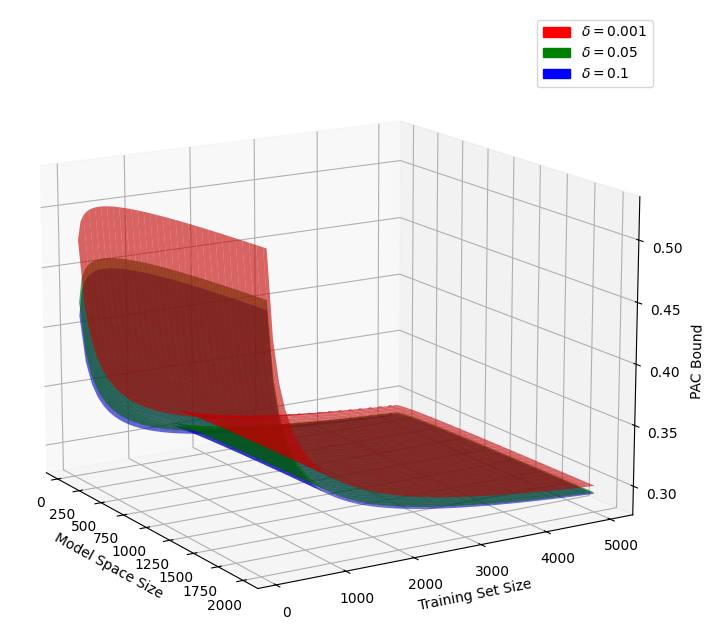
\includegraphics[width=\linewidth]{imgs/PAC_Bound.png}
        \end{figure}
        
    \end{minipage}

    \end{frame}
    }
    
    \begin{frame}{PAC Bound Proof Elements}
        The proof is based on:
        \begin{enumerate}
            \item \textbf{Chernoff's Inequality}: for any \(t > 0\),
            \[
                \mathbb{P}[U > s] = \mathbb{P}\left[e^{tU}>e^{ts}\right] \leq \frac{\mathbb{E}\left[e^{tU}\right]}{e^{ts}}\,.
            \]
            \item \textbf{The Union bound}:
            \[
                \mathbb{P}\left[ \sup_{1\leq i \leq M}  U_i\ > s\right] = \mathbb{P}\left[ \bigcup_{1\leq i \leq M} \{U_i > s\}\right] \leq \sum_{i=1}^M \mathbb{P}\left[ U_i > s\right]\,.
            \]
        \end{enumerate}
        \pause
        PAC-Bayes bounds are a generalization of the union bound argument that will allow us to deal with any parameter set \(\Theta\).
    \end{frame}

    \begin{frame}{What are PAC-Bayes Bounds?}
        A \textbf{data-dependent probability measure} is a function:
        \[
            \hat{\rho}: \bigcup_{n=1}^{\infty} (\mathcal{X} \times \mathcal{Y})^n \to \mathcal{P}(\Theta)\,.
        \]
        To get a \textbf{predictor}:
        \begin{enumerate}
            \item Draw a parameter \(\tilde{\theta} \sim \hat{\rho}\), \textbf{randomized estimator}.
            \item \textbf{Average} predictors
            \[
                f_{\hat{\rho}}(\cdot) := \mathbb{E}_{\theta \sim \hat{\rho}}[f_\theta(\cdot)]
            \]
        \end{enumerate}
    \end{frame}
    \begin{frame}
        With PAC-Bayes Bounds, we can obtain bounds related to
        \begin{enumerate}
            \item The risk of a randomized estimator, \(R(\tilde{\theta})\).
            \item The average risk of randomized estimators, \(\mathbb{E}_{\theta \sim \hat{\rho}}[R(\theta)]\).
            \item The risk of the aggregated estimator, \(R(f_{\hat{\rho}})\).
        \end{enumerate}
    \end{frame}

    {\setbeamercolor{background canvas}{bg=white}
    \begin{frame}{A first PAC-Bayes Bound}

    Let \(\pi \in \mathcal{P}(\Theta)\) be a \textbf{fixed} prob. measure (the prior), and \(\ell(\cdot, \cdot)\) be \textbf{bounded} in \([0, C]\).
    \pause

    \textbf{Cantoni's Bound, 2003}. For any \(\lambda > 0\), and any \(\delta \in (0,1)\),
    \[
    \mathbb{P}_S \left[ \forall \rho \in \mathcal{P}(\Theta), \ \mathbb{E}_{\theta \sim \rho}[R(\theta)] \leq \mathbb{E}_{\theta \sim \rho}[r(\theta)] + \frac{\lambda C^2}{8n} + \frac{\text{KL}(\rho|\pi) + \log\tfrac{1}{\delta}}{\lambda}\right] \geq 1-\delta\,.
    \]
    \begin{figure}
        \centering
        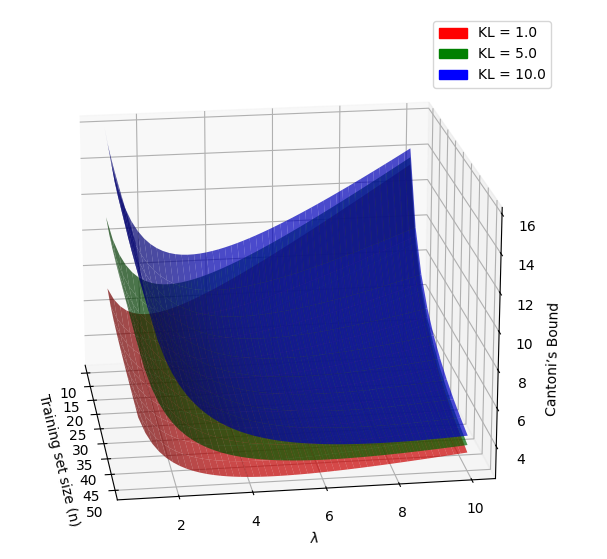
\includegraphics[width=0.35\linewidth]{imgs/cantoni.png}
        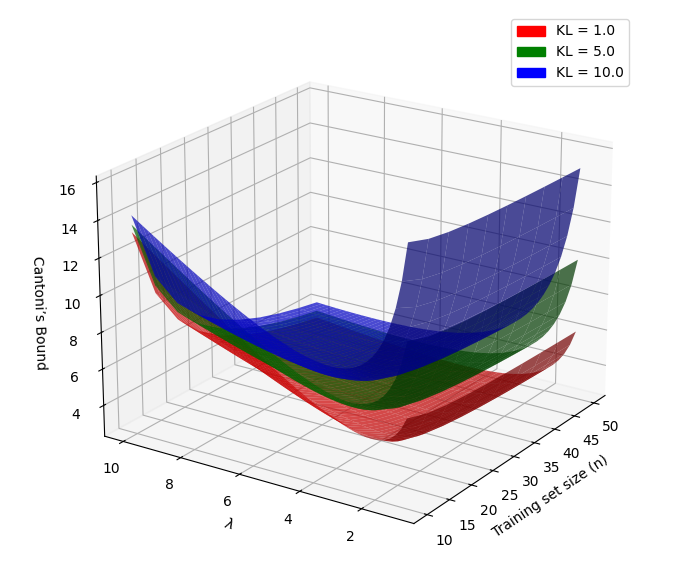
\includegraphics[width=0.37\linewidth]{imgs/cantoni2.png}
    \end{figure}
    \end{frame}
    }

    \begin{frame}{Gibbs Posterior}
        \[
            \hat{\rho}_\lambda := \argmin_{\rho \, \in \, \mathcal{P}(\Theta)} \left\{ \mathbb{E}_{\theta \sim \rho}[r(\theta)] + \frac{\text{KL}(\rho|\pi)}{\lambda} \right\}\,.
        \]
        Due to Donsker and Varadhan’s variational formula:
        \[
        \hat{\rho}_\lambda \propto e^{-\lambda r(\theta)}\pi(\theta)\,.
        \]
        \pause
        \[
            \text{If } \quad r(\theta) := -\ln P(S|\theta)\,, \quad \text{then, } \quad \hat{\rho}_\lambda \propto P(S|\theta)^\lambda\pi(\theta)\,.
        \]
        Related to \textbf{generalized} Bayesian framework and \textbf{tempered posteriors}.
        \pause
        \[
        \mathbb{P}_S \left( \mathbb{E}_{\theta \sim \hat{\rho}_\lambda}[R(\theta)] \leq \inf_{\rho \, \in \, \mathcal{P}(\theta)} \left[\mathbb{E}_{\theta \sim \rho}[r(\theta)] + \frac{\lambda C^2}{8n} + \frac{\text{KL}(\rho|\pi) + \log\tfrac{1}{\delta}}{\lambda}\right]\right) \geq 1-\delta\,.
        \]
    \end{frame}

    \begin{frame}{Order of Magnitude}
     Finite case \(\Theta = \{\theta_1, \dots, \theta_M\}\).
        \[
        \begin{aligned}
            \mathbb{E}_{\theta \sim \hat{\rho}_\lambda}[R(\theta)] &\leq \inf_{\rho \, \in \, \mathcal{P}(\theta)} \left[\mathbb{E}_{\theta \sim \rho}[r(\theta)] + \frac{\lambda C^2}{8n} + \frac{\text{KL}(\rho|\pi) + \log\tfrac{1}{\delta}}{\lambda}\right]\\\pause
            \Big[\text{D.V. formula}\Big] \quad &\leq -\frac{1}{\lambda}\log \sum_{\theta \, \in \, \Theta} \pi(\theta)e^{-\lambda r(\theta)} + \frac{\lambda C^2}{8n}+ \frac{\log \tfrac{1}{\delta}}{\lambda}\\\pause
            \left[e^{-\lambda r(\theta)} \leq e^{-\lambda \inf_{\eta \in \Theta}r(\eta)}\right] \quad &\leq \inf_{\theta \, \in\,  \Theta} \left[ r(\theta) + \frac{\log \frac{1}{\pi(\theta)}}{\lambda} \right] + \frac{\lambda C^2}{8n}+ \frac{\log \tfrac{1}{\delta}}{\lambda}
        \end{aligned}
        \]
        \pause
        Tight if \(r(\theta)\) and \(1/\pi(\theta)\) are \textbf{small simultaneously}; \(\pi\) cannot be large everywhere. The larger \(\Theta\), the more ``spread'' \(\pi\) is.
    \end{frame}

    \begin{frame}
        \[
        \begin{aligned}
            \mathbb{E}_{\theta \sim \hat{\rho}_\lambda}[R(\theta)] \leq \inf_{\theta \, \in \,\Theta} \left\{r(\theta) + \frac{\log \frac{1}{\pi(\theta)\delta }}{\lambda} + \frac{\lambda C^2}{8n} \right\}
        \end{aligned}
        \]
        If we choose an uniform prior \(\pi(\theta) = 1/M\), the optimal \(\lambda = \sqrt{8n \log(M/\delta)/C^2}\)

        \[
        \mathbb{P}_S\left( \mathbb{E}_{\theta \sim \hat{\rho}_\lambda}[R(\theta)] \leq \inf_{\theta \, \in \, \Theta} \ \{r(\theta)\} + C \sqrt{\frac{\log \tfrac{M}{\delta}}{2n}}\right) \geq 1-\delta\,.
        \]
        \pause
        \begin{enumerate}
            \item The Gibbs posterior \(\hat{\rho}_\lambda\) satisfies the \textbf{same bound as the ERM}.
            \item However \(\hat{\rho}_\lambda\) and \(\hat{\theta}_{ERM}\) are \textbf{not} equivalent! 
            \item The PAC-Bayes bound \textbf{can be tighter}. 
        \end{enumerate}
    \end{frame}

    \begin{frame}{Dirac Delta Posteriors}
        \textbf{Cantoni's Bound, 2003}. For any \(\lambda > 0\), and any \(\delta \in (0,1)\),
        \[
        \mathbb{P}_S \left( \forall \rho \in \mathcal{P}(\Theta), \ \mathbb{E}_{\theta \sim \rho}[R(\theta)] \leq \mathbb{E}_{\theta \sim \rho}[r(\theta)] + \frac{\lambda C^2}{8n} + \frac{\text{KL}(\rho|\pi) + \log\tfrac{1}{\delta}}{\lambda}\right) \geq 1-\delta\,.
        \]

        It holds for every \(\rho \in \mathcal{P}(\Theta)\). Then, consider a fixed parameter \(\theta\) and \(\delta_\theta \in \mathcal{P}(\Theta)\).\pause
        \begin{enumerate}
            \item \(\mathbb{E}_{\eta \sim \delta_{\theta}}[r(\eta)] = r(\theta)\).
            \item \(\text{KL}(\delta_{\theta}|\pi) = -\log \pi(\theta)\).
        \end{enumerate}
        \[
            \mathbb{P}_S \left( \forall \theta \in\Theta, \ R(\theta) \leq r(\theta) + \frac{\lambda C^2}{8n} + \frac{\log\tfrac{1}{\delta} + \log\tfrac{1}{\pi(\theta)}}{\lambda}\right) \geq 1-\delta\,.
        \]
    \end{frame}
    \begin{frame}
        \[
            \mathbb{P}_S \left( \forall \theta \in\Theta, \ R(\theta) \leq r(\theta) + \frac{\lambda C^2}{8n} + \frac{\log\tfrac{1}{\delta} + \log\tfrac{1}{\pi(\theta)}}{\lambda}\right) \geq 1-\delta\,.
        \]
        Taking the infimum over \(\theta\) with \(\Theta = \{\theta_1, \dots, \theta_M\}\):
        \[
            R(\hat{\theta}_{ERM}) \leq \inf_{\theta\,  \in\,  \Theta} \ \{r(\theta)\} + \frac{\lambda C^2}{8n} + \frac{\log\tfrac{M}{\delta}}{\lambda}\,.
        \]
        Taking again \(\lambda = \sqrt{8n \log(M/\delta)/C^2}\)
        \[
            R(\hat{\theta}_{ERM}) \leq \inf_{\theta \, \in\,  \Theta} \ \{r(\theta)\} +C\sqrt{\frac{\log\tfrac{M}{\delta}}{2n}}\,.
        \]
    \end{frame}

    \begin{frame}{Remarks}
        \begin{enumerate}[<+->]
            \item PAC-Bayes can be used to prove \textbf{generalization bounds for Gibbs posteriors}.
            \item  Recent papers study \textbf{non-Bayesian robust estimators} of the mean and covariance matrix of \textbf{heavy-tailed} random vectors.
            \item The choice of \(\lambda\) has a different status:
            \begin{enumerate}
                \item Bound on the ERM: \(\lambda\) is chosen to \textbf{minimize the bound}, but the estimation procedure is not affected by \(\lambda\).
                \item Bound for the Gibbs posterior is also minimized with respect to \(\lambda\), but \(\hat{\rho}_\lambda\) \textbf{depends on} \(\lambda\).
            \end{enumerate}
        \end{enumerate}
        
    \end{frame}

    \begin{frame}{Example: Lipschitz loss and Gaussian prior}
        \textbf{Assumptions}:
        \begin{enumerate}
            \item \(\Theta = \mathbb{R}^d\).
            \item \(\theta \mapsto \ell(f_\theta(x), y)\) is \(L\)-Lipschitz for any \((x, y)\).
            \item \(\pi(\theta) = \mathcal{N}(0, \sigma^2 I_d)\).
        \end{enumerate}
        \pause
        \textbf{Starting point}:
        \[
            \forall \rho \in \mathcal{P}(\Theta), \ \mathbb{E}_{\theta \sim \rho}[R(\theta)] \leq \mathbb{E}_{\theta \sim \rho}[r(\theta)] + \frac{\lambda C^2}{8n} + \frac{\text{KL}(\rho|\pi) + \log\tfrac{1}{\delta}}{\lambda}\,.
        \]
        \pause
        \textbf{Simplifications}:
        \[
            \text{KL}(\rho|\pi) = \frac{\|m\|^2}{2\sigma ^2} + \frac{d}{2}\left[ \frac{s^2}{\sigma^2} + \log \frac{\sigma ^2}{s^2} - 1 \right]\,.
        \]
        \[
            r(\theta) \text{ is } L\text{-Lipschitz}\implies \mathbb{E}_{\theta \sim \rho}[r(\theta)] \leq r(m) + Ls\sqrt{d}\,.
        \]
    \end{frame}
    \begin{frame}
        \[
        (\tilde{m}, \tilde{s}) = \argmin_{m\in \mathbb{R} ^d, \ s > 0} \left\{ r(m) + \frac{\lambda C^2}{8n} + \frac{\frac{\|m\|^2}{2\sigma^2} + \frac{d}{2}\left[ \frac{s^2}{\sigma^2} + \log \frac{\sigma^2}{s^2} - 1 \right] + \log \frac{1}{\delta}}{\lambda}\right\}\,.
        \]
        
        \[
        \tilde{\rho}_\lambda := \mathcal{N}(\tilde{m}, \tilde{s}^2I_d) \text{ is a variational approximation of } \hat{\rho}_\lambda\,.
        \]
    \end{frame}

    \begin{frame}{The choice of \(\lambda\)}
        In general, is \textbf{not possible} to optimize the right-hand side of the PAC-Bayes equality \textbf{with respect to} \(\lambda\).
        
        \pause
        
        The \textbf{optimal value} of \(\lambda\) could depend on \(\rho\).
        
        \pause
        
        A natural idea is to propose a \textbf{finite grid} \(\Lambda \subset (0, +\infty)\) and to minimize over this grid, which can be justified by a \textbf{union bound argument}:
                \[
        \mathbb{P}_S \left[ \forall \rho \in \mathcal{P}(\Theta), \ \mathbb{E}_{\theta \sim \rho}[R(\theta)] \leq \mathbb{E}_{\theta \sim \rho}[r(\theta)] + \frac{\lambda C^2}{8n} + \frac{\text{KL}(\rho|\pi) + \log\tfrac{\text{card}(\Lambda)}{\delta}}{\lambda}\right] \geq 1-\delta\,.
        \]
    \end{frame}

    \begin{frame}{Final Remarks}
        \begin{enumerate}
            \item Optimizing \(\rho\) and \(\lambda\) is an \textbf{open-problem}.
            \item ``There is no PAC-Bound tight for \textbf{all data-generating distributions}'' --- Gastpar et al., \textit{Fantastic generalization measures are nowhere to be found}, ICLR (2024).\pause
            \[\downarrow\]
            \begin{center}
            Data-distribution dependent or Algorithm dependent bounds
            \end{center}
            \item PAC-Bayes Bounds for \textbf{unbounded} losses are an open problem.
        \end{enumerate}
    \end{frame}

    \begin{frame}[standout]
        Thank you for your {\color{magenta}attention}!
    \end{frame}

    \begin{frame}[allowframebreaks]
    \nocite{*}
    \printbibliography[heading=none]
    \end{frame}

    \begin{frame}{Kullback-Leibler Divergence}

    Given two probability measures \(\mu\) and \(\nu\) in \(\mathcal{P}(\Theta)\), the Kullback-Leibler (or simply KL) divergence between \(\mu\) and \(\nu\) is defined as
    \[
    \text{KL}(\mu| \nu) = \int \log \left(\frac{d\mu}{d\nu}(\theta) \right) \mu d(\theta)
    \]
    Under absolutely continuity assumptions:
    \[
    \text{KL}(\mu| \nu) = \int \mu (\theta) \log \left(\frac{\mu(\theta)}{\nu(\theta)} \right) \ d(\theta)\,.
    \]
    \end{frame}

    \begin{frame}{Hoeffding's Inequality}
        Let \(X_1, X_2, \dots, X_n\) be independent random variables such that \(a_i \leq X_i \leq b_i\) almost surely. Then, consider
        \[
            S_n = X_1 + \dots + X_n\,.
        \]
        It verifies that
        \[
        P(S_n - \mathbb{E}[S_n]) \geq t) \leq \exp \left( \frac{2t^2}{\sum_{i = 1}^n (b_i - a_i)^2} \right)\,.
        \]
    \end{frame}

    \begin{frame}{Donsker and Varadhan’s Variational Formula}
        For any measurable, bounded function \(h : \Theta \to \mathbb{R}\) we have:
        \[
            \log \mathbb{E}_{\theta \sim \pi}[e^{h(\theta)}] = \sup_{\rho \, \in\, \mathcal{P}(\Theta)} \left[ \mathbb{E}_{\theta \sim \rho}[h(\theta)] - \text{KL}(\rho | \pi) \right]\,.
        \]
        It verifies that
        \[
        P(S_n - \mathbb{E}[S_n]) \geq t) \leq \exp \left( \frac{2t^2}{\sum_{i = 1}^n (b_i - a_i)^2} \right)\,.
        \]
    \end{frame}
    
\end{document}